\documentclass[twoside,11pt]{article}

%%%%% PACKAGES %%%%%%
\usepackage{pgm2016}
\usepackage{amsmath}
\usepackage{algorithm}
\usepackage[noend]{algpseudocode}
\usepackage{subcaption}
%\usepackage[utf8]{inputenc}		%NOT USED?
\usepackage[english]{babel}		%NOT USED?
\usepackage{paralist}			%NOT USED?
\usepackage[lowtilde]{url}
\usepackage{fixltx2e}
\usepackage{listings}
\usepackage{color}
\usepackage{hyperref}

\usepackage{auto-pst-pdf}
\usepackage{pst-all}
\usepackage{pstricks-add}



%%%%% MACROS %%%%%%
\algrenewcommand\Return{\State \algorithmicreturn{} }
\algnewcommand{\LineComment}[1]{\State \(\triangleright\) #1}
\renewcommand{\thesubfigure}{\roman{subfigure}}
\definecolor{codegreen}{rgb}{0,0.6,0}
\definecolor{codegray}{rgb}{0.5,0.5,0.5}
\definecolor{codepurple}{rgb}{0.58,0,0.82}
\definecolor{backcolour}{rgb}{0.95,0.95,0.92}
\lstdefinestyle{mystyle}{
   backgroundcolor=\color{backcolour},  
   commentstyle=\color{codegreen},
   keywordstyle=\color{magenta},
   numberstyle=\tiny\color{codegray},
   stringstyle=\color{codepurple},
   basicstyle=\footnotesize,
   breakatwhitespace=false,        
   breaklines=true,                
   captionpos=b,                    
   keepspaces=true,                
   numbers=left,                    
   numbersep=5pt,                  
   showspaces=false,                
   showstringspaces=false,
   showtabs=false,                  
   tabsize=2
}
\lstset{style=mystyle}

%%%%% SHORT HEADING %%%%%%
% Short headings should be running head and authors last names
\ShortHeadings{Parallel Solution for Message Passing on Arithmetic Circuits}{dos Santos}
\firstpageno{1}

\begin{document}

\title{Research Task C - The Problem: \\ Parallel Solution for Message Passing on Arithmetic Circuits}

\author{\name Andr\'e E. dos Santos \email dossantos@cs.uregina.ca \\
\addr Department of Computer Science \\
University of Regina \\ 
Regina, Canada
}



\maketitle

\begin{abstract}%   <- trailing '%' for backward compatibility of .sty file
Arithmetic Circuits (AC) is a graphical method for reasoning with Bayesian networks (BNs) based on partial differentiation.
ACs is a viable framework for applications of BNs to embedded systems, which are characterized for their primitive computational resources. 
An AC is a directed acyclic graph with four types of variables: evidence indicators, network parameters (probability values), sum nodes and product nodes.
There are two phases to compile the AC: upward and inward.
Those phases pass messages through the AC, which are essentially numbers.
The number of messages passed in both phases is twice the number of edges in the compilation of the polynomial.
Once the BN is processed, one can compute in constant-time answers to a large class of probabilistic queries.
In this paper we present the algorithm to compile the AC.
We show how a parallel solution and describe how it compares to a serial solution.
%
%
%BNs is a probabilistic graphical model for dealing with uncertainty in artificial intelligence.
%However, BNs are known for requiring a high amount of processing during its running time of execution.
%This strongly limits the applications of BNs to embedded systems, which are characterized for their primitive computational resources. 
%\cite{darwiche00} proposes a new approach for inference in Bayesian networks based on partial differentiation.
%Once the BN is processed, one can compute in constant-time answers to a large class of probabilistic queries.
%One of the key contributions is the possible cost-effective implementation on a variety of software and hardware platforms.
%
%The paper has a mathematical heavy notation and it is not a easy reading.
%A reason is the weak background on probabilistic graphical models.
%Thus, it is not self contained, which means one might have to look for second sources.
%Throughout the paper, several advantages are presented
%All claims have proof and are sound.
%However, some points are not discussed in the paper, such the generalization of the proposed approach for other networks.
\end{abstract}


\section{Introduction}
\label{sec:intro}


Bayesian networks (BNs) \citep{pear88} is a probabilistic graphical model for dealing with uncertainty in artificial intelligence.
%BNs overcame the acquisition intractability problem when reasoning with the a join probability distribution.
However, BNs are known for requiring a high amount of processing during its running time of execution \citep{koll09}.
This strongly limits the applications of BNs to embedded systems, which are characterized for their primitive computational resources. 
%Due those limitations, consumer electronics often utilizes semantic weaker frameworks, such as Fuzzy logic or ruled-based systems.
\cite{darwiche00} proposed a new approach for inference in Bayesian networks based on partial differentiation called \emph{Arithmetic Circuits} \citep{darwiche00}.
The differential approach presents two key contributions.
First, it enphasizes the role of partial differentiation on probabilistic reasoning, giving a new utility to central tasks of BNs.
Second, it helps the migration of BN applications to embedded systems, which are known for constraint in computational resources.

An AC is a directed acyclic graph with four types of variables: evidence indicators, network parameters (probability values), sum nodes and product nodes.
The leaves are evidence indicators ands network parameters and the rest of the graph consists of sum and product nodes.
%The AC is build according to the elimination ordering of the inference algorithm variable elimination. 
There are two phases to compile the AC given and evidence: upward and inward.
%The first phase consists of following the operators numbers upward.
By the end of the upward phase we can compute the probability of the evidence.
By the end of the downward phase we can compute in constant-time answers to a large class of probabilistic queries.

In this paper we present the algorithm to compile an AC.
It computes both upward and inward phase.
We show how a parallel solution and describe how it compares to a serial solution.
There are limitations to the solutions since those steps are constrained by a topological ordering.

This paper is organized as follows.
In Section \ref{sec:background}, arithmetic circuits are reviewed.
Section \ref{sec:eval} presents the parallel solution for message passing on arithmetic circuits.
Conclusions are given in Section \ref{sec:conc}.


\section{Background}
\label{sec:background}

A \emph{joint probability distribution} (JPD) is function $P$ on the Cartesian product $V$ of the variable domains such that the following two conditions hold: 
\begin{align}
	&0 \leq P(v) \leq 1.0\text{ for each configuration $v \in V$; and}\\		
	&\sum_{v \in V}{P(v)} = 1.0
\end{align}

%Unlike \emph{fuzzy logic} and \emph{rule-based systems}, probability theory provides a rigorous mathematical foundation for the representation of uncertainty and for reasoning with uncertainty.
%However, acquisition intractability is one of the problems of using only the jpd to model the problem domain.
%For instance, specifying one probability value would be difficult with 50 variables, let alone 2\textsuperscript{50} probability values.

%By exploiting the notion of \emph{probabilistic conditional independence}, \cite{pear88} solved the jpd acquisition problem by introducing Bayesian networks.
A \emph{Bayesian network} (BN) \cite{pear88} is a directed acyclic graph (DAG) on finite set of discrete variables $U$ together with \emph{conditional probability tables} (CPTs) $P(v_1 | Pa(v_1))$, $P(v_2|Pa(v_2))$, $\ldots$, $P(v_n|Pa(v_n))$,
where $Pa(v_i)$ denotes the parents of the variable $v_i$ in the DAG.
The product of the CPTs for the DAG on $U$ is a \emph{joint probability distribution} $P(U)$ \citep{pear88}.
For example, Figure \ref{fig:bn} shows a Bayesian network with CPTs $P(a)$ and $P(b|a)$ in Table 1.


\begin{figure}[htbp]
\centering
 \psset{unit=1cm}
      \begin{pspicture}(0,0.5)(2,3)%\showgrid
        \rput(2,1){\ovalnode{X1}{$B$}}
        \rput(0,1){\ovalnode{X2}{$A$}}
        
        \ncline{->}{X2}{X1}
         
  \end{pspicture}
%\includegraphics[page=1]{amidst_T41-pics.pdf}
\caption{A BN from \citep{darwiche00}.}
\label{fig:bn}
\end{figure}


%Unfortunately, both exact and approximate inference in Bayesian networks are, in general, \emph{NP-hard} \citep{koll09}. 
%Thus, the use of exponential complexity algorithms is justified.
%That implies a limitation for BN applications to embedded systems, which are known for constraint in computational resources.

A \emph{parameterized} CPT receives a evidence indicator $\lambda$ multiplied to the probability value.
For instance, Table 2 shows the parameterized CPTs for the BN of Table 1.
Notice that $\bar x$ denotes the instantiation $x = 0$.

\begin{table}[!htb]
    \label{subtb:pa}
    \caption{Table (a) provides the prior probability of variable $A$ and Table (b) provides the conditional probability of $B$ given $A$.}
    \begin{subtable}{.5\linewidth}
      \centering
        \caption{}
        \begin{tabular}{c|c}
            $A$ & $P(A)$ \\ \hline
            1 & 0.3 \\
            0 & 0.7
        \end{tabular}
    \end{subtable}%
    \begin{subtable}{.5\linewidth}
      \centering
        \caption{}
        \begin{tabular}{cc|c}
            $A$ & $B$ & $P(B|A)$ \\ \hline
            1 & 1 & 0.1 \\
            1 & 0 & 0.9 \\
            0 & 1 & 0.8 \\
            0 & 0 & 0.2 \\
        \end{tabular}
    \end{subtable} 
\end{table}




%In this section we show the mains ideas proposed by the paper ``A Differential Approach to Inference in Bayesian Networks'' \citeyearpar{darwiche00}.
%We give an overview on how to  represent a BN as a polynomial, and then compiling and evaluating the polynomial representation.

%\subsection{Polynomial Representation of Bayesian networks}

%An AC is a directed acyclic graph with four types of variables: evidence indicators, network parameters (probability values), sum nodes and product nodes.
%The leaves are evidence indicators ands network parameters and the rest of the graph consists of sum and product nodes.
%The AC is build according to the elimination ordering of the inference algorithm variable elimination. 
%There are two phases to compile the AC given and evidence: upward and inward.
%%The first phase consists of following the operators numbers upward.
%By the end of the upward phase we can compute the probability of the evidence.
%By the end of the downward phase we can compute in constant-time answers to a large class of probabilistic queries.

A BN can be represented as a polynomial $\cal F$ as follows:
\begin{align}
	{\cal F}(\lambda,\theta) = \sum_{U}{\prod{\theta_i}\prod{\lambda_i}}
\end{align}

As an example, the polynomial of the BN in Figure 1 is

\begin{align}
	{\cal F} = \theta_{A}\theta_{B|A}\lambda_{A}\lambda_{B} +
	  \theta_{A}\theta_{\bar{B}|A}\lambda_{A}\lambda_{\bar{B}} +
	 \theta_{\bar{A}}\theta_{B|\bar{A}}\lambda_{\bar{A}}\lambda_{B} +
	  \theta_{\bar{A}}\theta_{\bar{B}|\bar{A}}\lambda_{\bar{A}}\lambda_{\bar{B}}
\end{align}

The size of the polynomial is exponential to the size of the network.

%Now, with a evidence we can set a indicator $\lambda$ to either 0 or 1.
%If is consistent with the evidence is 1, and is 0 otherwise.
%For example, if the evidence is $A\bar{B}$ that is, $A$ is true, $B$ is false, then
%	${\cal F}(
%	\lambda_{A}=1,
%	\lambda_{\bar{A}}=0,
%	\lambda_{B}=0,
%	\lambda_{\bar{B}}=1,
%	\theta_{A} = 0.3,
%	\theta_{\bar{A}} = 0.7,
%	\theta_{B|A} = 0.1,
%	\theta_{\bar{B}|A} = 0.9,
%	\theta_{B|\bar{A}} = 0.8,
%	\theta_{\bar{B}|\bar{A}} = 0.2,			
%	)$,
%which equal to 0.27 in this case.
%The probability values are the correspondents in the respectively CPTs.
%Therefore, the polynomial is a linear function of many variables, where each one corresponds to either an evidence indicator $\lambda$ or a probability value $\theta$.
%Each parameter has degree one.
%For each instantiation given an evidence, the polynomial can be evaluated to compute the probability of the variable given the evidence.

%The author highlights that BNs represented by polynomial function has been already exploited by other authors \citep{castillo1996goal,castillo1997sensitivity,russell1995local}.
%However, the evidence indicators were fixed to a particular value.
%Hence, they  could not be used to answer queries with respect to varying evidence.


%\subsection{Compiling a Bayesian networks}

%The paper presents a algorithm, called $\Call{VE\_COMPLETE}{}$, to compile a polynomial representation of a BN. 
%$\Call{VE\_COMPLETE}{}$ receives as input a BN and an elimination ordering of the variables.
%The result is a more compact polynomial following the elimination ordering used to construct this new presentation.
Following an elimination ordering of variables, an AC can be drawn for the compiled polynomial.
For instance, the compiled polynomial in (4) is
\begin{eqnarray}
	{\cal F} = \theta_{A}\lambda_{A}(\theta_{B|A}\lambda_{B} + \theta_{\bar{B}|A}\lambda_{\bar{B}}) + \theta_{\bar{A}}\lambda_{\bar{A}}(\theta_{B|\bar{A}}\lambda_{B}+\theta_{\bar{B}|\bar{A}}\lambda_{\bar{B}})
\end{eqnarray}
and depicted in Figure \ref{fig:comp}.

\begin{figure}[!htb]
    \begin{center}
    	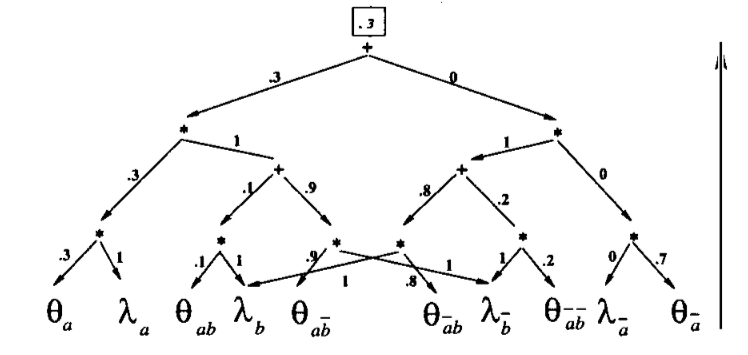
\includegraphics[width=\columnwidth]{figures/compiled.png}
		\caption{An AC representing Equation (5).}
		\label{fig:comp}
    \end{center}
\end{figure}


\section{Evaluating and Differentiating a Polynomial Representation}
\label{sec:eval}

The evaluation of the AC and computing the partial derivatives is a two-phase message passing scheme in which each message is simply a number.
The first phase, massages are sent from nodes to their parents in the AC following the operations of each node.
The phase starts from the leaves up to the root.
Note that the value of a of a node can not be computed before all its children values has been computed.
First phase is described in lines 1-11 in Algorithm 1.
Figure \ref{fig:comp} shows this process, where it leads to assigning the value 0.3 to the root, indicating that the probability of evidence $E$ is $P(E) = 0.3$.

Second phase, messages are sent from nodes to children in the same rooted DAG, leading to computation of all partial derivatives.
This process is known as \emph{back propagation} \cite{rumelhart1988learning}, a common method of training artificial neural networks, and its proven to be able to compute the partial derivatives of variables on the leaves.
The phase starts from the root down to the leaves.
The derivative value of the root, by definition, is always 1.
For the remaining nodes $v$, if the parent $Pa(v)$ is a summation node, the derivative value of $v$ is equal to its parent.
If the parent $Pa(v)$ is a multiplication node, the derivative value of $v$ is equal to the summation of its parent times the others siblings of $v$.
This processes is illustrated in Figure \ref{fig:deri}.
Note that the derivative of a node of a node can not be computed before all its parents derivatives has been computed.
Second phase is described in lines 13-27 in Algorithm 35.

\begin{figure}[!htb]
    \begin{center}
    	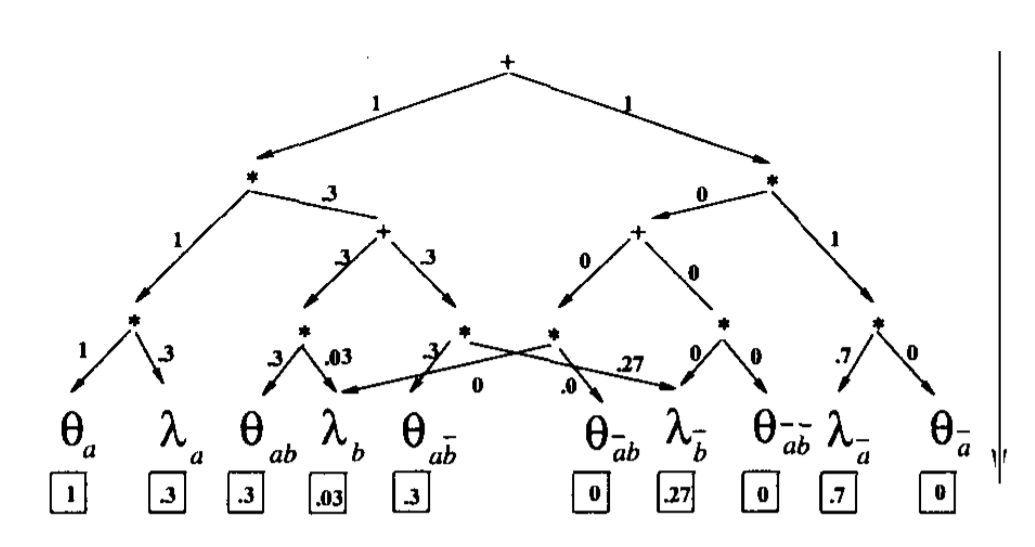
\includegraphics[width=\columnwidth]{figures/deriv.png}
		\caption{Second phase of the evaluation of AC in Figure 5, under evidence $E=A$.}
		\label{fig:deri}
    \end{center}
\end{figure}

\begin{figure}[!htb]
    \begin{center}
    	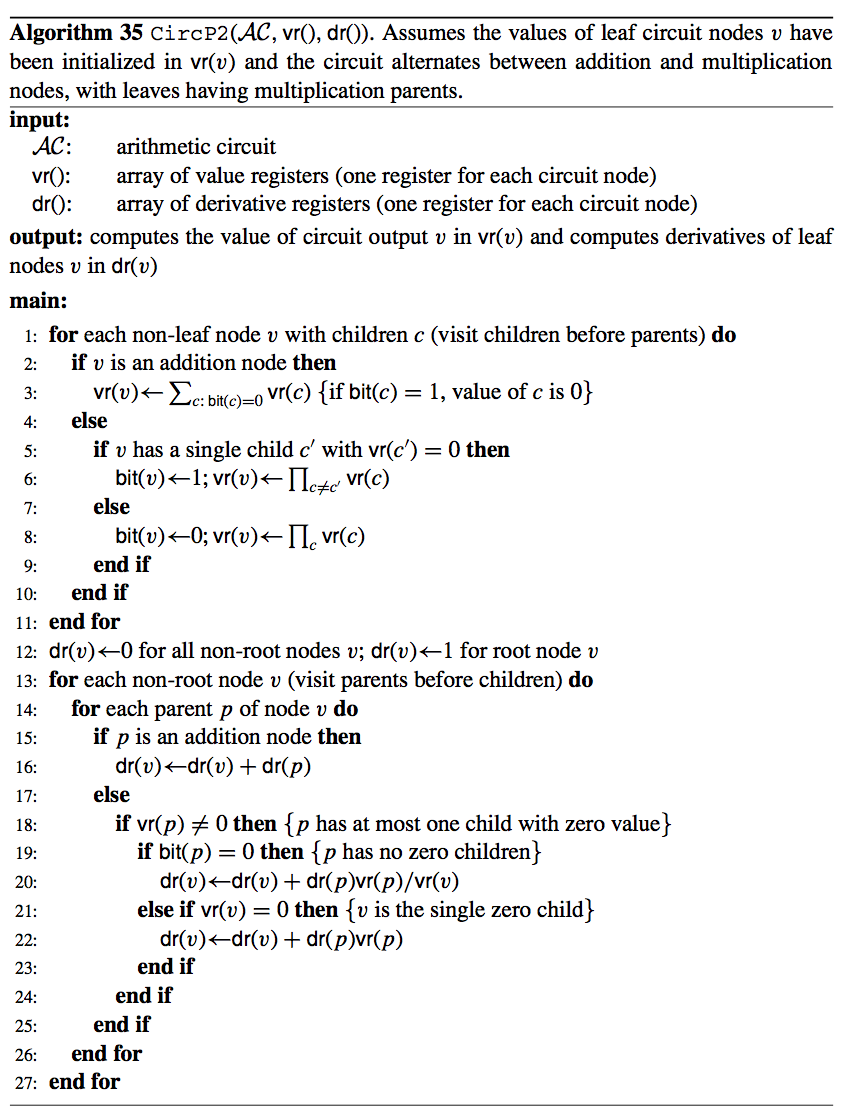
\includegraphics[width=\columnwidth]{figures/alg.png}
%		\caption{}
		\label{fig:alg}
    \end{center}
\end{figure}

After the two-phase steps we have the capacity to answer, in constant time, a very large class of probabilistic queries, relating to classical inference, parameter estimation, model validation and sensitivity analysis.
Some of those queries are
(i) in the root node the probability of the evidence, and 
(ii) the posterior marginal of any network variable.

\subsection{Serial Solution}

The serial solution computes the values and derivatives of each node sequentially in both cases.
The only restrictions are those imposed by the topological ordering.
For instance, the second phase where the derivatives are propagated top-bottom, can be implemented with \emph{breadth-first search} algorithm.

\subsection{Parallel Solution}

The phases of evaluating and differentiating an AC can improved by the parallelization of the nodes value calculation.
Phase one, massages are sent from nodes to their parents in the AC following the operations of each node, as described in lines 1-11 in Algorithm 1.
Since the phase starts from the leaves up to the root, the layers of operations (sum and product) can be computed in parallel.
For instance, in the second last layer of Figure \ref{fig:comp}, the value of nodes 
($\theta_a \star \lambda_a$), 
($\theta_{ab} \star \lambda_{{b}}$), 
($\theta_{a{\bar b}} \star \lambda_{{\bar b}}$),
($\lambda_{{b}} \star \theta_{{\bar a}b}$),
($\lambda_{{\bar b}} \star \theta_{{\bar a}\bar{b}}$), and
($\lambda_{{\bar a}} \star \theta_{{\bar a}}$) 
can be computed in parallel.


In the second phase, messages are sent from nodes to children in the same rooted DAG, leading to computation of all partial derivatives, as described in lines 12-27 in Algorithm 1.
Since the phase starts from the root down to the leaves, the derivatives of the layers of children can be computed in parallel.
For instance, in the last layers of Figure \ref{fig:deri}, the derivatives of  nodes 
$\theta_a $,
$\lambda_a$,
$\theta_{ab}$,
$\lambda_{{b}}$,
$\theta_{a{\bar b}}$,
$\theta_{{\bar a}b}$,
$\lambda_{{\bar b}}$,
$\theta_{\bar{a}\bar{b}}$,
$\lambda_{{\bar a}}$, and
$\theta_{{\bar a}}$
can be computed in parallel.
 
\section{Conclusion}
\label{sec:conc}

Reasoning with ACs presents several advantages.
It emphasizes the role of partial differentiation on probabilistic reasoning, giving a new utility to central tasks of BNs.
Also, it helps the migration of BN applications to embedded systems, which are known for constraint in computational resources.


There are two phases to compile the AC: upward and inward.
Once the BN is processed, one can compute in constant-time answers to a large class of probabilistic queries.
In this paper we presented the algorithm to compile the AC, drawn from \cite{darwiche2009modeling}.
It computes both upward and inward phase.
We have shown how a parallel solution can be implemented and described how it compares to a serial solution.
The limitations to the solutions are essentially imposed by  topological ordering only.


\vskip 0.2in
\bibliography{references/references}
\end{document}
